\textbf{Trefethen 7.2}

Solve the boundary value problem $u_{xx} + 4u_x + e^x u = \sin{(8x)}$ numerically on $[-1, 1]$ with boundary 
conditions $u(-1) = u(1) = 0$. To ten digits of accuracy, what is $u(0)$?

\begin{solution}
  The first 15 iterations of our spectral method solution and corresponding values at $x = 0$ are given by the output
  of \texttt{problem\_5.m} below:

  \begin{figure}[h]
    \begin{subfigure}[b]{0.9\textwidth}
      \begin{verbatim}
            u(0) = 0.00476307074
            u(0) = 0.00848395571
            u(0) = 0.00937809416
            u(0) = 0.00955676355
            u(0) = 0.00959055326
            u(0) = 0.00959681652
            u(0) = 0.00959796822
            u(0) = 0.00959817930
            u(0) = 0.00959821793
            u(0) = 0.00959822499
            u(0) = 0.00959822629
            u(0) = 0.00959822652
            u(0) = 0.00959822656
            u(0) = 0.00959822657
            u(0) = 0.00959822657
      \end{verbatim}
    \end{subfigure}
    \begin{subfigure}[b]{0.9\textwidth}
      \centering
      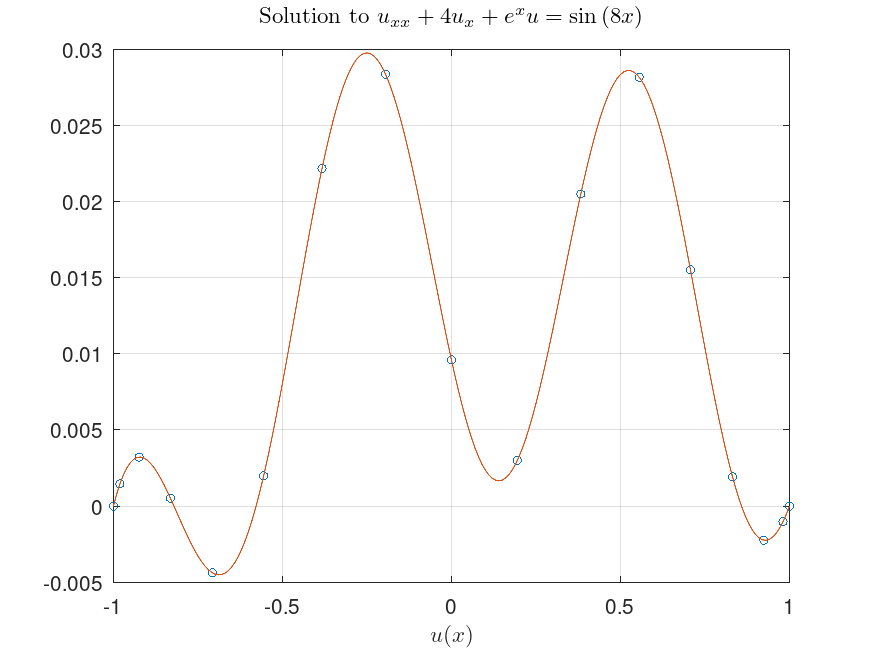
\includegraphics[width=0.8\textwidth]{problem_5.png}
    \end{subfigure}
    \caption{Iterative solution to $u_{xx} + 4u_x + e^x u = \sin{(8x)}$ with Dirichlet BCs.}
    \label{fig:bvp_problem_5}
  \end{figure}
  \ \\
\end{solution}